\begin{center}
  \Large
  \textbf{BIOGRAFI PENULIS}
\end{center}

\addcontentsline{toc}{chapter}{BIOGRAFI PENULIS}

\vspace{2ex}

\begin{wrapfigure}{L}{0.3\textwidth}
  \centering
  \vspace{-3ex}
  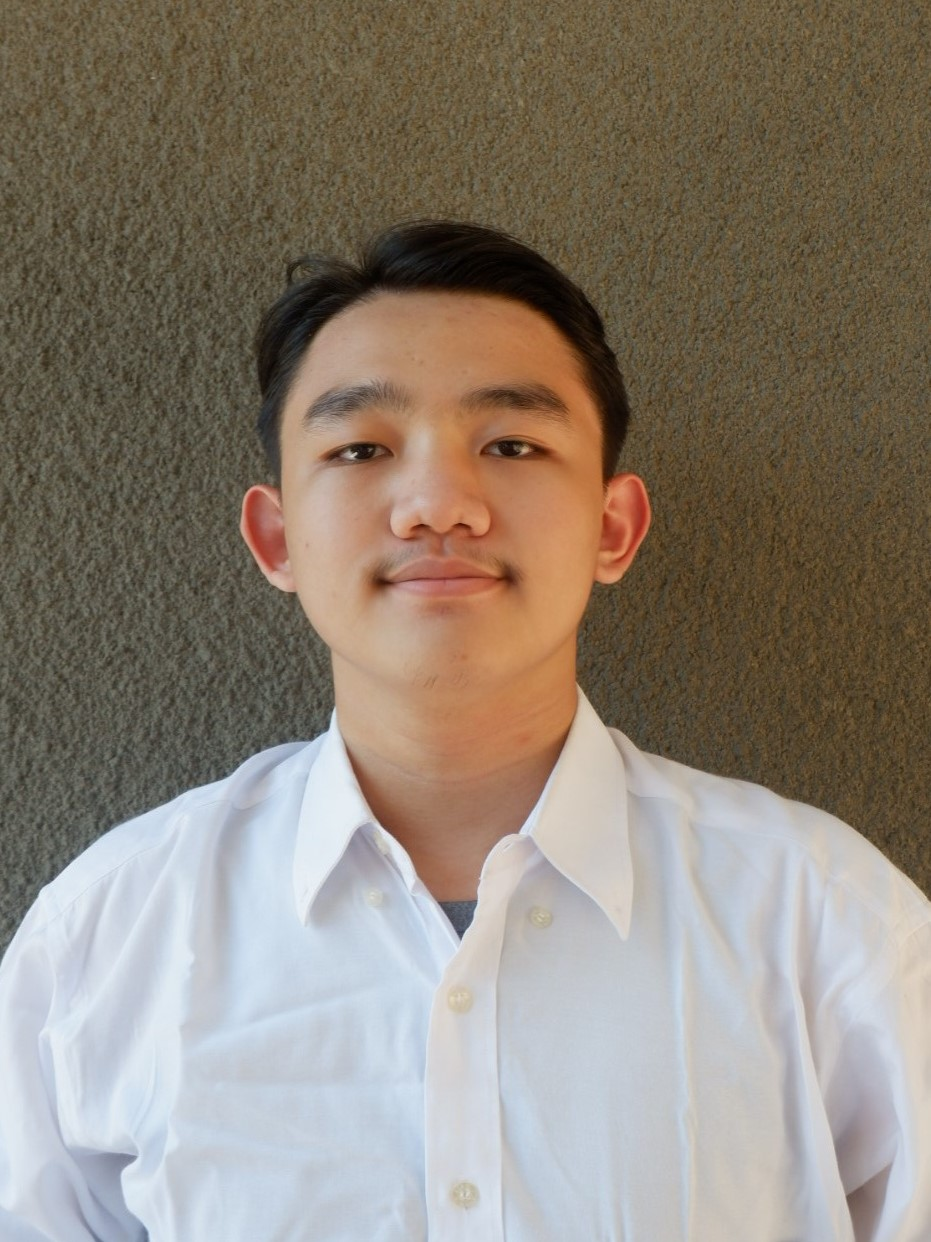
\includegraphics[width=0.3\textwidth]{gambar/Steven_Figo_3x4.jpeg}
  \vspace{-4ex}
\end{wrapfigure}

Steven Figo lahir di Sibolga, 30 November 2004, merupakan anak pertama dari tiga bersaudara. Penulis telah menempuh pendidikan formal yaitu di TK Tri Ratna Sibolga, SD Tri Ratna Sibolga, SMP Tri Ratna Sibolga, dan SMAS Tri Ratna Sibolga. Setelah lulus dari SMAS Tri Ratna Sibolga pada tahun 2022 penulis mengikuti SBMPTN dan diterima di Departemen Teknologi Informasi FTEIC - ITS pada tahun 2022 dan terdaftar dengan NRP 5027221021.

Di lingkungan Departemen Teknologi Informasi, penulis merupakan pengurus Himpunan Mahasiswa Teknologi Informasi (HMIT) dan pernah berkontribusi sebagai panitia dalam ajang tahunan ARA 4.0, 5.0, dan 6.0. Pada bidang kompetisi, penulis pernah menjadi finalis Gemastik 2024 pada kategori Smart City. Selain itu, penulis juga aktif sebagai asisten mata kuliah untuk subjek Sistem Operasi, Komunikasi Data dan Jaringan Komputer, Internet of Things (IoT), Kecerdasan Artifisial dan Machine Learning, Struktur Data \& Pemrograman Berorientasi Objek, Strategi Optimasi Komputasi Awan, serta Smart City.

Di luar aktivitas akademik, penulis juga aktif mengembangkan diri melalui UKM Paduan Suara Mahasiswa ITS. Sebagai anggota, penulis telah mengikuti berbagai kompetisi tingkat nasional maupun internasional, termasuk meraih medali emas pada ajang Karangturi International Choir Competition, Fespa UBAYA, dan Malaysian Choral Eisteddfod.
